\chapter{Used Technologies}\label{sec:technologies}
In this chapter I will briefly present technologies that were used during development
 and I will explain why these technologies were used.

\section{Platform}
In the following section I will describe technologies that were used for building cloud platform.
These technologies enabled us to build a scalable solution with easy deployment.

\IDEA{Time consuming installation, build once use many times}
\IDEA{We want to make installation process as fast as possible}
\IDEA{
  Compare Docker with Virtualbox/Vagrant

  Initially a virtual machine with all dependencies installed was used.
  Even though this satisfied all deployment requirements it does not seem useful,
    because this solution had much larger performance overhead
    and it does not allow to control the application at such fine grain level as Docker.
}

The most important tool used during development is \textbf{Docker}
  -- a portable, lightweight application runtime and packaging tool\footnote{
  \url{http://www.docker.com}
}.
It means that it allows to specify environment in which we want to run a process.
The environment is described in a Dockerfile,
  see Figure~\ref{fig:dockerfile} for an example.
From a Dockerfile Docker builds an image which is later used to run that process.
All dependencies are stored in the image and this image can be used on different machines.
Therefore deployment time is much lower.

As a result only required dependency for running CloudASR is Docker
  because all other dependencies are already installed in the Docker images.
Additionally, it removes bugs caused by different versions of libraries used in development and production environmnent
  because developers can use the same images in both environments.

\begin{figure}
  \verbatiminput{snippets/Dockerfile}

  \label{fig:dockerfile}
  \caption{An example of Dockerfile.}
  \TODO{add better caption}
\end{figure}


\IDEA{server crashes, manage all servers}
\TODO{cite Mesos: A Platform for Fine-Grained Resource Sharing in the Data Center}
The tool that allows CloudASR to run on many machines is \textbf{Mesos}.
It lets users program against set of machines like it is a single machine.
That means that we can create set of servers and run application on them.
Also, Mesos supports Docker so images that are used in development can be also used on Mesos cluster.
Furthermore, Mesos takes care about high availability of the platform.
Thus, whenever some part of the CloudASR crashes Mesos will try to fix that.

\textbf{Marathon}\footnote{\url{https://mesosphere.github.io/marathon/}} is a framework built on top of Mesos whose main responsibility is to launch long running applications.
It also takes care about high availability (when an application crashes it tries to restart it)
  and easy scalability (running instances can be scaled in one click).
Finally, it has a web user interface (see Figure~\ref{fig:marathon}) and REST API,
  through which applications can be started, scaled or stopped.

\begin{figure}
  \centering
  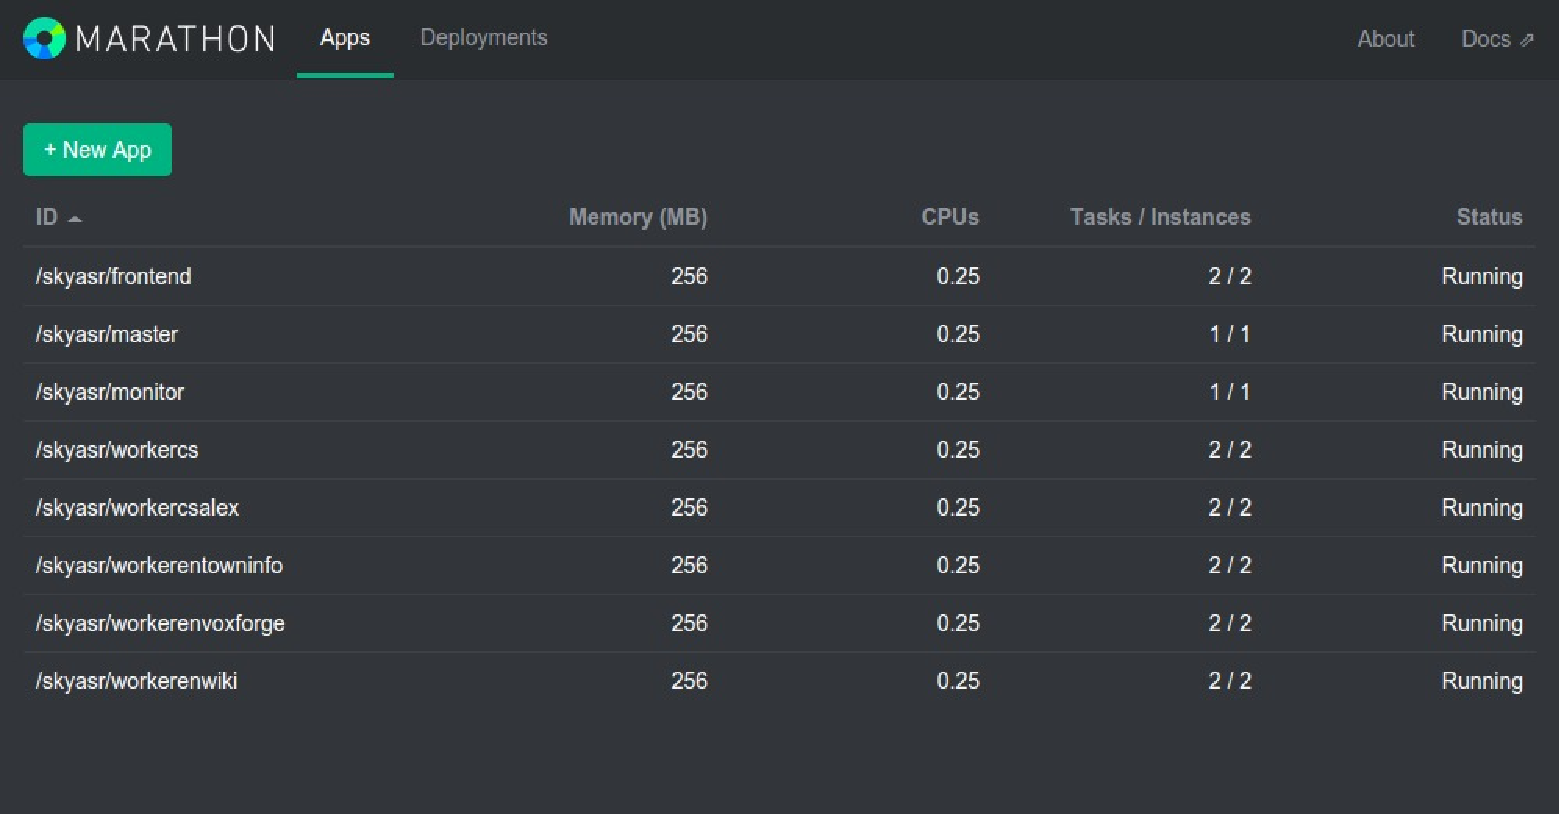
\includegraphics[width=0.95\textwidth]{./img/marathon.pdf}

  \label{fig:marathon}
  \caption{\TODO{An example of marathon}}
  \TODO{Describe screenshot better}
\end{figure}

Since the traffic of CloudASR platform can be very large,
  it is not possible to process all HTTP requests on one machine.
Therefore, there must be a load-balancer to distribute workload between running instances.
CloudASR platform uses \textbf{HAProxy}\footnote{\url{http://www.haproxy.org/}} load-balancer,
  but any other load-balancers can also used with appropriate setup.


\section{Continuos Integration \& Delivery}
During development of CloudASR I obeyed several practises,
  namely Continuous Integration and Continuous Delivery.
In order to be able to do that I had to setup a platform which consisted of \textbf{Jenkins-CI}\footnote{\url{https://jenkins-ci.org/}} and \textbf{Docker Registry}\footnote{\url{https://github.com/docker/docker-registry}}.

The most important tool for Continous Integration \& Delivery of CloudASR is Jenkins-CI.
It watches CloudASR git repository
  and whenever a new code is pushed into this repository it schedules a new build of the platform.
During this build the most recent code is pulled from the repository and then the docker images are built.
After that tests are run to check that the new code did not break anything.
Finally, successfully built images are tagged with current build number and pushed to the Docker Registry.


Docker Registry is a repository of Docker images.
Even though, there are several Docker Registry providers\footnote{\url{https://hub.docker.com/}, \url{https://quay.io/}},
  which are free for open-source projects,
  CloudASR uses its own free Docker Registry,
  in order to be also able to use proprietary software that cannot be shared with public.


\section{Backend}
The main programming language used for development is \textbf{Python}\footnote{\url{https://www.python.org/}}.
Web and REST API are built on top of \textbf{Flask}\footnote{\url{http://flask.pocoo.org/}} microframework
  and they use \textbf{Gunicorn}\footnote{\url{http://gunicorn.org/}} for production deployment.

\IDEA{Flask - plugins, lightweight, support for SocketIO}
\IDEA{Gunicorn - performance, support for SocketIO...}

Because CloudASR architecture consists of several nodes which need to communicate between each other.
For this communication ClousASR uses \textbf{ZeroMQ}\footnote{\url{http://zeromq.org/}},
  because of its simple design, high performance and support for every modern language.
Moreover usage of ZeroMQ makes it possible to implement each node in different programming language if needed.
With ZeroMQ it is possible to create many messaging patterns,
  but CloudASR uses only two: request-reply and push-pull.
These patterns are described in detail on Figure~\ref{fig:zeromq}.

\TODOIMG{fig:zeromq}{Description of used ZeroMQ patterns.}

In order to be able to send complex messages via ZeroMQ sockets, messages have to be serialized.
Initially, CloudASR used JSON for serialization because of its simplicity and its support in almost every language,
  but suddenly I found out that JSON does not support serialization of binary data,
  therefore, I had to choose another serialization format.
As a result, CloudASR uses \textbf{Google Protocol Buffers}\footnote{\url{https://developers.google.com/protocol-buffers/}},
  which has support in many languages,
  allows specification of various message types (See Figure~\ref{fig:protobuf} for example)
  and serializes messages in very compact way
  (See Table~\ref{fig:protobuf-benchmark} for a comparison of different serializations).

\begin{table}[h]
  \begin{tabular}{rrl}
  \textbf{raw file size} & 56146 & \\
  \cline{1-3}
  \textbf{bytes\_protobuf} & 56118 & 0.999x \\
  \textbf{base64} & 74872 & 1.333x \\
  \textbf{json\_array} & 158590 & 2.824x \\
  \end{tabular}

  \label{fig:protobuf-benchmark}
  \caption{\TODO{add better description}}
\end{table}

\begin{figure}
  \verbatiminput{snippets/protobuf.proto}

  \label{fig:protobuf}
  \caption{An example of Google Protocol Buffer message specification.}
  \TODO{Add beter caption}
\end{figure}


\section{Frontend}
Frontend uses several well-known open-source libraries, namely,
  \textbf{Twitter Bootstrap}\footnote{\url{http://getbootstrap.com/2.3.2/}} for CSS styling of the web,
  \textbf{jQuery}\footnote{\url{https://jquery.com/}}
  and \textbf{Angular.js}\footnote{\url{https://angularjs.org/}} for interactive elements on the web.

\TODOIMG{fig:demo}{CloudASR Web Demo}

Modern web browsers supports \textbf{WebAudio API}\footnote{\url{http://webaudio.github.io/web-audio-api/}},
  which is a high-level JavaScript API for processing and synthesizing audio in web applications.
One of the things that can be done with this API is recording of an audio.
Thus, it is possible to create a web demo for CloudASR online speech recogniser.
The demo is based on \textbf{Recorder.js}\footnote{\url{https://github.com/mattdiamond/Recorderjs}} library,
  which can record output of WebAudio API and return it as a PCM chunks.

Next step is to send these chunks to the API.
Because the demo demonstrates the online speech recognition mode,
  it is not possible to wait for whole recording to be recorded and then send it to the API via HTTP POST request,
  thus, CloudASR uses \textbf{Socket.IO}\footnote{\url{http://socket.io/}} to send stream of chunks to the API
  and to receieve stream of results from the API.
